
\section{$p$-Laplacian equation}

FIXME for $p>1$,
    $$I[u] = \int_\Omega \frac{1}{p} |\grad u|^p - fu$$
the variational equation is the weak form of a PDE:
\begin{align*}
I[u+\eps v] - I[u] &= \int_\Omega \frac{1}{p} |\grad u + \eps \grad v|^p + \frac{1}{p} |\grad u|^p - \eps f v \\
   &= \eps \left(\int_\Omega |\grad u|^{p-2} \grad u \cdot \grad v - f v\right) + O(\eps^2)
\end{align*}
so we want
    $$0 = \int_\Omega |\grad u|^{p-2} \grad u \cdot \grad v - f v$$
for all $v \in W^{1,p}_0(\Omega)$.  this can become a strong form by another integration by parts,
    $$0 = - \Div\left(|\grad u|^{p-2} \grad u\right) - f$$
which is \eqref{poissonsquare} if $p=2$

\section{Structured $Q^1$ finite elements}

FIXME

\begin{marginfigure}
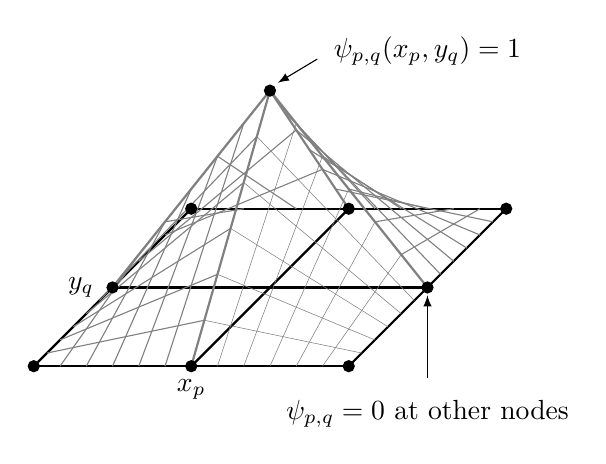
\begin{tikzpicture}[scale=0.5]

  % strong grid around elements
  \draw[thick] (0,0) -- (8,0);
  \draw[thick] (2,2) -- (10,2);
  \draw[thick] (4,4) -- (12,4);
  \draw[thick] (0,0) -- (4,4);
  \draw[thick] (4,0) -- (8,4);
  \draw[thick] (8,0) -- (12,4);

  \def\ytop{7};

  % tent lines
  \draw[gray,thick] (6,\ytop) -- (4,0);
  \draw[gray,thick] (6,\ytop) -- (2,2);
  \draw[gray,thick] (6,\ytop) -- (10,2);
  \draw[gray,thick] (6,\ytop) -- (8,4);

  \def\dx{(10.0-6.0)/6};
  \def\dy{(2.0-\ytop)/6};
  \foreach \jj in {1,...,5}
  {
       \draw[gray,very thin] ({6+\jj*\dx},{\ytop+\jj*\dy}) -- ({4+(4/6)*\jj},0.0);
  }

  \def\dx{(4.0-6.0)/6};
  \def\dy{(0.0-\ytop)/6};
  \foreach \jj in {1,...,5}
  {
       \draw[gray,very thin] ({6+\jj*\dx},{\ytop+\jj*\dy}) -- ({10-(2/6)*\jj},{2-(2/6)*\jj});
  }

  \def\dx{(2.0-6.0)/6};
  \def\dy{(2.0-\ytop)/6};
  \foreach \jj in {1,...,5}
  {
       \draw[gray,thin] ({6+\jj*\dx},{\ytop+\jj*\dy}) -- ({4-(4/6)*\jj},0.0);
  }

  \def\dx{(4.0-6.0)/6};
  \def\dy{(0.0-\ytop)/6};
  \foreach \jj in {1,...,5}
  {
       \draw[gray,thin] ({6+\jj*\dx},{\ytop+\jj*\dy}) -- ({2-(2/6)*\jj},{2-(2/6)*\jj});
  }

  \def\dx{(10.0-6.0)/6};
  \def\dy{(2.0-\ytop)/6};
  \foreach \jj in {1,...,5}
  {
       \draw[gray,thin] ({6+\jj*\dx},{\ytop+\jj*\dy}) -- ({8+(4/6)*\jj},4.0);
  }

  \def\dx{(8.0-6.0)/6};
  \def\dy{(4.0-\ytop)/6};
  \foreach \jj in {1,...,5}
  {
       \draw[gray,thin] ({6+\jj*\dx},{\ytop+\jj*\dy}) -- ({10+(2/6)*\jj},{2+(2/6)*\jj});
  }

  \def\dx{(2.0-6.0)/3};
  \def\dy{(2.0-\ytop)/3};
  \foreach \jj in {1,...,2}  % reduce clutter
  {
       \draw[gray,thin] ({6+\jj*\dx},{\ytop+\jj*\dy}) -- ({8-(4/3)*\jj},4.0);
  }

  \def\dx{(8.0-6.0)/3};
  \def\dy{(4.0-\ytop)/3};
  \foreach \jj in {1,...,2}
  {
       \draw[gray,thin] ({6+\jj*\dx},{\ytop+\jj*\dy}) -- ({2+(2/3)*\jj},{2+(2/3)*\jj});
  }

  % nodes in base plane
  \filldraw (0,0) circle (4pt);
  \filldraw (4,0) circle (4pt);
  \filldraw (8,0) circle (4pt);
  \filldraw (2,2) circle (4pt);
  %\filldraw (6,2) circle (4pt);   % (x_j,y_k) is at (6,2)
  \filldraw (10,2) circle (4pt);
  \filldraw (4,4) circle (4pt);
  \filldraw (8,4) circle (4pt);
  \filldraw (12,4) circle (4pt);

  % node at tent top
  \filldraw (6,\ytop) circle (4pt);

  % annotate
  \draw (10,\ytop+1.0) node {$\psi_{p,q}(x_p,y_q)=1$};
  \draw[-latex] (7.2,\ytop+0.8) -- (6.2,\ytop+0.2);
  \draw (10,-1.2) node {$\psi_{p,q}=0$ at other nodes};
  \draw[-latex] (10,-0.3) -- (10,1.8);

  % label center point
  \draw (4,-0.6) node {$x_p$};
  \draw (1.2,2) node {$y_q$};

\end{tikzpicture}

\caption{FIXME}
\label{fig:q1hat}
\end{marginfigure}

FIXME code uses \texttt{SNESSetObjective()} only, though also \texttt{SNESSetFunction()}; no hand-made Jacobian at all

FIXME try NCG


\section{Exercises}

\renewcommand{\labelenumi}{\arabic{chapter}.\arabic{enumi}\quad}
\renewcommand{\labelenumii}{(\alph{enumii})}
\begin{enumerate}
\item FIXME
\end{enumerate}